%-------------
% PACKAGES %%
%-------------
\documentclass[12pt]{article}
\usepackage[english]{babel}
\usepackage[utf8x]{inputenc}
\usepackage{amsmath}
\usepackage{float}
\usepackage{hyperref}
\usepackage{graphicx}
\usepackage{listings}
\usepackage[colorinlistoftodos]{todonotes}
\usepackage[nottoc,numbib]{tocbibind}
\usepackage[parfill]{parskip}
\usepackage{changepage}
\usepackage{subcaption}
\usepackage{changepage}
\usepackage{listings}
\usepackage{color}
\usepackage[htt]{hyphenat}
%\usepackage{minted}

\definecolor{dkgreen}{rgb}{0,0.6,0}
\definecolor{gray}{rgb}{0.5,0.5,0.5}
\definecolor{mauve}{rgb}{0.58,0,0.82}

\lstset{%frame=tb,
  language=C,
  aboveskip=3mm,
  belowskip=3mm,
  showstringspaces=false,
  columns=flexible,
  basicstyle={\small\ttfamily},
  numbers=none,
  numberstyle=\tiny\color{gray},
  keywordstyle=\color{blue},
  commentstyle=\color{dkgreen},
  stringstyle=\color{mauve},
  breaklines=false,
  breakatwhitespace=false,
  tabsize=4,
  morekeywords={FIR_H_BUFFER,dsp16_t,dsp16_filt_iirpart}
}

\lstset{emph={%  
    DSP16_Q,H_SIZE%
    },emphstyle={\color{mauve}}%
}

\title{Hochschule Bonn-Rhein-Sieg}

\begin{document}

%-------------------------
%	uncomment irrelevant 
%	parts, like logo etc
%-------------------------
\pagenumbering{Alph}
\begin{titlepage}

\newcommand{\HRule}{\rule{\linewidth}{0.5mm}} % Defines a new command for the horizontal lines, change thickness here

\begin{center}
%---------------------
%	HEADING SECTIONS
%---------------------
\textsc{\LARGE Hochschule Bonn-Rhein-Sieg}\\[1.5cm] % Name of your university/college
\textsc{\Large Multi-Agent and Agent Systems}\\[0.5cm] % Major heading such as course name
\textsc{\large Team : Right brothers}\\[0.5cm] % Minor heading such as course title

%------------------
%	TITLE SECTION
%------------------
\HRule \\[0.4cm]
{ \huge \bfseries German Bakery}\\[0.4cm] % Title of your document
\HRule \\[1.5cm]
 
%--------------------
%	AUTHOR SECTION
%--------------------
 %\begin{minipage}{1.4\textwidth}
 %\begin{flushleft} 

\large\emph{Authors:}\\ Arun Rajendra Prabhu\\ Dharmin Bakaraniya\\ Md Zahiduzzaman\\[1.0cm]%
%\large\emph{Collaborated with:}\\Collaborator\\[1cm]
                        		% \\ [1.0cm]%

 %\end{flushleft}
 %\end{minipage}

%---------------------
%	Supervisor
%---------------------
 %\begin{minipage}{0.4\textwidth}
 %\begin{flushright} \large
 %\emph{Supervisor:} \\
 %Dr. James \textsc{Smith} % Supervisor's Name
 %\end{flushright}
 %\end{minipage}\\[2cm]

% If you don't want a supervisor, uncomment the two lines below and remove the section above
%\Large \emph{Author:}\\
%John \textsc{Smith}\\[3cm] % Your name

{\large \today}\\[1cm] % Date

%----------
%	LOGO 
%----------

\includegraphics[width=3.7in]{Logo.png}\\%[1cm]
\end{center}
\end{titlepage}
\pagenumbering{arabic}
\pagebreak
%-------------------------
%	Table of Contents
%-------------------------
\tableofcontents
\pagebreak
%-------------------------
%       Main Text
%-------------------------
\section*{Introduction:}

The overall architecture diagram describing the deligation of tasks in the bakery is provided by the figure~\ref{fig:1}.

\begin{figure}[H]
  \centering
  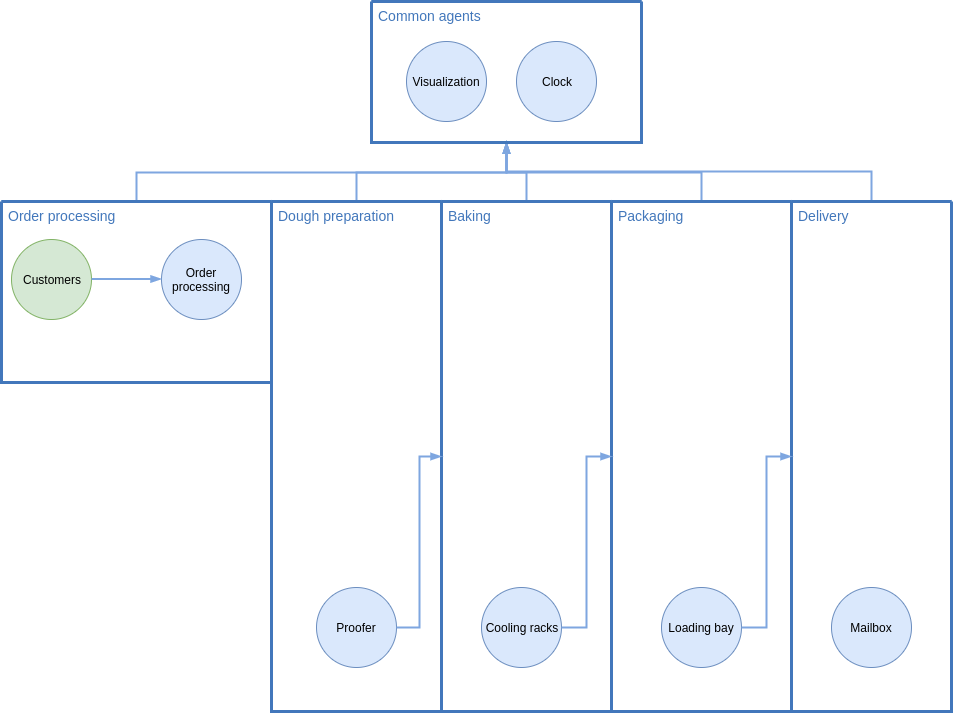
\includegraphics[width=0.8\textwidth]{Architecture.png}
  \caption{Architecture Diagram}
  \label{fig:1}
\end{figure}

The right brothers team was responsible to provide the \textbf{baking} and \textbf{packaging} stages. In addition to these stages, it was also responsible for providing the \textbf{base agent}, \textbf{time keeper} agent and \textbf{board visualization} feature. These agents fall in the common agents catagory and we will look at each one of them in detail in the coming sections.

With figure~\ref{fig:1} as the starting point, we created a component diagram, figure~\ref{fig:2} to describe the relationship between the agents in different stages. This diagram was created from the perspective of the stages which are under the right brother's responsibility, hence the only the interface agents of the other stages are represented in the diagram.
 
\begin{figure}[H]
  \centering
  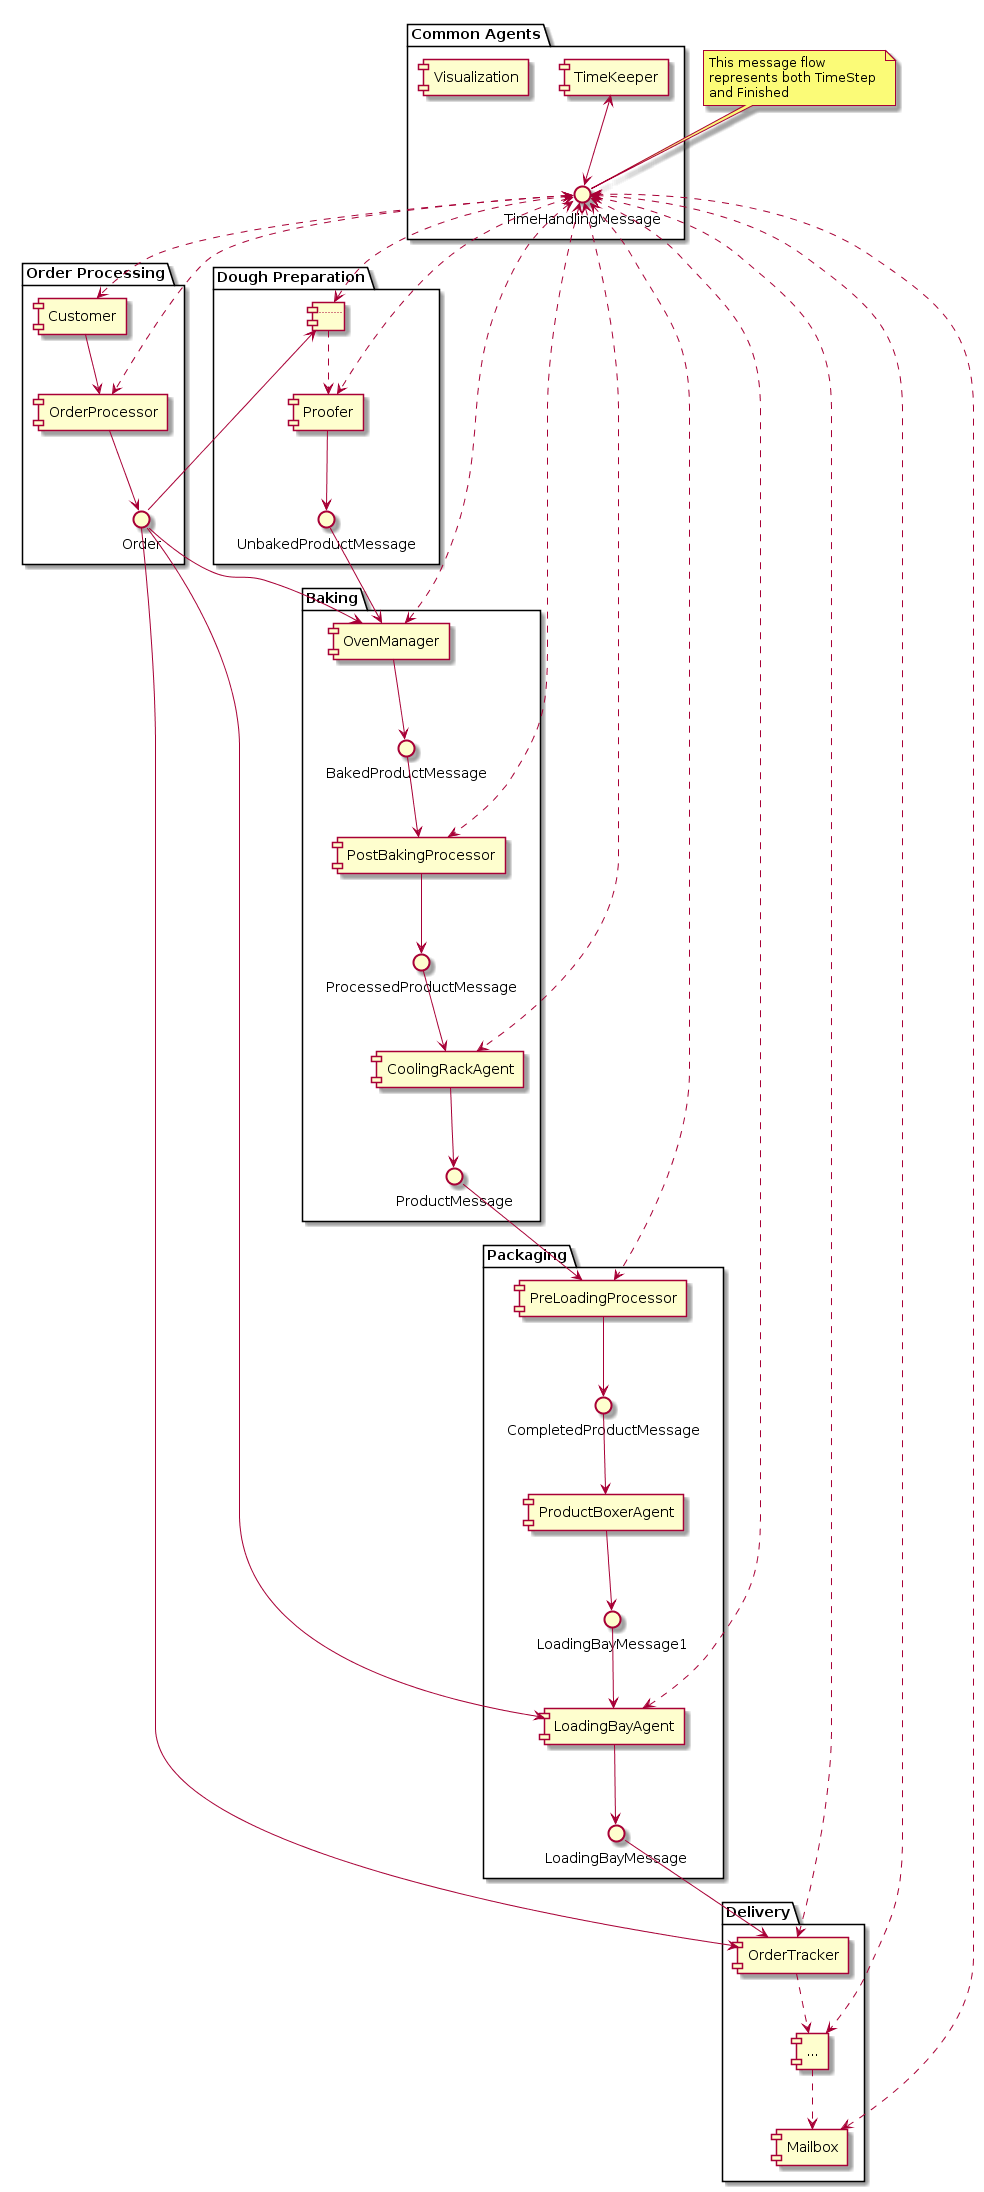
\includegraphics[width=0.7\textwidth]{component_diagram.png}
  \caption{Component diagram representation}
  \label{fig:2}
\end{figure}

All the agents in our stages are created statically at startup. 
To illustrate this decision, consider the baking stage. Each bakery has a fixed number of ovens. In our design, we have a single agent called as OvenManager looking after all the ovens. Hence as per our design, it does not make sense to use dynamic agent creation for OvenManager. Also static agent creation, simplifies the overall interoperability to a cetain extent.
\section{Baking Stage:}
\begin{itemize}
    \item \textbf{OvenManager}: 
 We assign a single Agent to manage all the ovens in the bakery.
 It receives the \texttt{Order} from \texttt{OrderProcessor} agent. 
 It receives \texttt{UnbakedProductMessage} from \texttt{Proofer}.
 It bakes the products it received from \texttt{Proofer} and sends \texttt{BakedProductMessage} to \texttt{PostBakingProcessor}.
 It aggregates products of same type if the product is not being baked. 
    \item \textbf{PostBakingProcessor}:
 It receives \texttt{BakedProductMessage} from \texttt{OvenManager}.
 It processes all the steps in the recipe of that product which occur between \texttt{Baking} and \texttt{Cooling} steps. 
 It sends the \texttt{ProcessedProductMessage} to \texttt{CoolingRackAgent}.
    \item \textbf{CoolingRackAgent}:
 It receives \texttt{ProcessedProductMessage} from \texttt{PostBakingProcessor}.
 It performs cooling step of the recipe corresponding to that product.
 It sends \texttt{ProductMessage} to \texttt{PreLoadingProcessor} in the packaging stage.
\end{itemize}
\section{Packaging Stage:}
\begin{itemize}
    \item \textbf{PreLoadingProcessor}:
 It recieves \texttt{ProductMessage} from \texttt{CoolingRackAgent} from Baking stage.
 It performs all steps in recipe of that product which lie between \texttt{Cooling} and \texttt{Packaging}.
 It sends \texttt{CompletedProductMessage} to \texttt{ProductBoxerAgent}.
	\item \textbf{ProductBoxerAgent}: It receives \texttt{CompletedProductMessage} from the \texttt{PreLoadingProcessor}. It also receives the \texttt{Order} from \texttt{OrderProcessor}. It then prioritizes the orders based on the delivery times. It supports two types of priorities,
\begin{itemize}
\item Hard priority: Waits for the entire order of higher priority is completed before it moves on to process the next high priority order.
\item Soft priority: Checks if the products available in the inventory can be used to satisfy the pending orders according to their priority. If suppose there are 5 donuts in inventory and order1(high priority) needs 10 donuts and order2(lower priority) needs 5 donuts, then the 5 donuts are used to satisfy order2. However if there were 10 donuts in the inventory then the 10 donuts would have been used to satisfy order1.\
\end{itemize}
\texttt{LoadingBayMessage} is sent to the \texttt{LoadingBay} agent under two conditions,
\begin{itemize}
\item If a box is filled.
\item If a box is not full, however, all the required number of items of a product type in an order have been received.
\end{itemize}
    \item \textbf{LoadingBayAgent}:
 It recieves \texttt{LoadingBayMessage} from \\ \texttt{ProductBoxerAgent}.
 It then checks for order completion. If any orders are complete, it sends the  message to the \texttt{OrderTracking/OrderAggregator} agent of the \texttt{Delivery Stage}.   
\end{itemize}

\section{Common Agents:}
\begin{itemize}
    \item \textbf{TimeKeeper}: 
 It is responsible for the movement of time in the entire bakery eco-system.
 This is responsible for providing all the other agents with a common time reference so that everyone are in sync except the visualization agents.
 This also gets feedback from all the agents about the status of their tasks.
 If all the agents are done with whatever task they were supposed to finish in the time step, the TimeKeeper increments the time step. 
 It is also responsible for shutting down the platform when the simulation time ends.
\item \textbf{BaseAgent}:
BaseAgent is a parent to all agents in bakery simulation.
It is mainly responsible for registering the agent to yellow pages and talking to TimeKeeper.
It is also responsible for sending the message to visualization agents.
Every agent that inherits BaseAgent has to call \texttt{finished} when their task is finished for that time step.
\item \textbf{Visualization}:
Visualization agent receives messages from baseAgent of all agents and parses this message to extract whetever information it needs.
It then uses this information to create graphical representation using \texttt{JavaFX}.
\end{itemize}

\bibliography{refs}
\bibliographystyle{IEEEtran}

\end{document}